\chapter{Intro-opgaver}

\begin{figure}[h!]
\centering
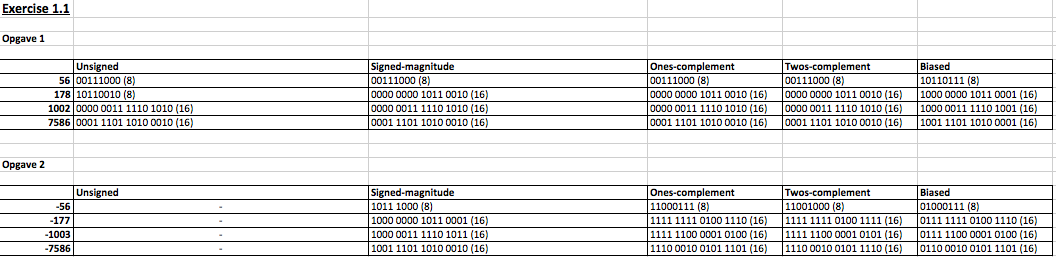
\includegraphics[scale=0.3]{figs/Ex1.png}
\caption{Exercise 1.1}
\label{fig:Ex1.1}
\end{figure}

\begin{figure}[h!]
\centering
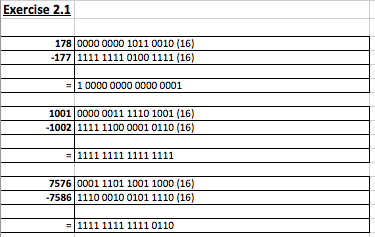
\includegraphics[scale=0.6]{figs/Ex2.png}
\caption{Exercise 2.1}
\label{fig:Ex2.1}
\end{figure}

\begin{figure}[h!]
\centering
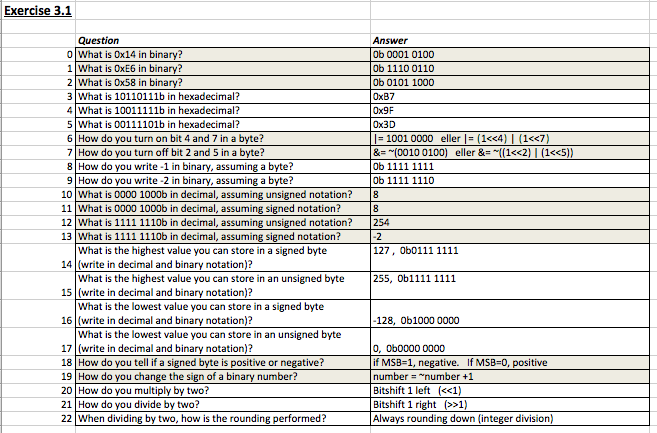
\includegraphics[scale=0.6]{figs/Ex3.png}
\caption{Exercise 3.1}
\label{fig:Ex3.1}
\end{figure}

\begin{figure}[h!]
\centering
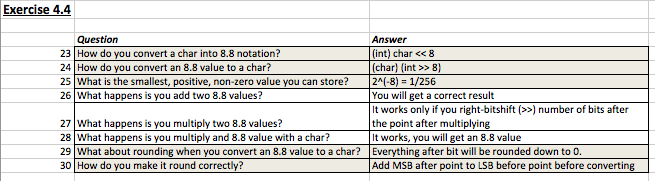
\includegraphics[scale=0.6]{figs/Ex4.png}
\caption{Exercise 4.4}
\label{fig:Ex4.4}
\end{figure}
